% 1) Title
% 2) Date
% 3) Location
% 4) Present
% 5) Picture
% 6) Start Time
% 7) Stop Time
\insertmeeting 
	{Building Day} 
	{07/21/21}
	{Hagerty High School}
	{Nathan, Samantha}
	{Images/RobotPics/robot.jpg}
	{12:00}
  {3:00}
	
\section*{Hardware}
\noindent\hfil\rule{\textwidth}{.4pt}\hfil
\subsection*{Goals}
\begin{itemize}
    \item Build New mecanum drivetrain   

\end{itemize} 

\noindent\hfil\rule{\textwidth}{.4pt}\hfil

\subsection*{Accomplishments}
This meeting we put together all of the parts we designed so far to build our new mecanum drivetrain. This drivetrain uses GoBilda's thin mecanum wheels driven by 2 andymark Neverest motors connected to the wheels using pullies and 2 htd belts. We used these specfic wheels because they are one of the only companies that creates a thin wheel while maintining the size we want; they also have an extremely easy attachment system which fufills our assembly goal we have this season. The drivetrain driveplates were designed to be made out of metal, but we prototyped them with wood before we go through the more expensive process of cutting them out of metal with a CNC router. We still have to finish assembling the drivetrain, but in exciting news this meeting was also the first in person meeting for one of our new members! Because we were in person, we were able to show the new kids around the robotics room and demo power tools like the drill press and belt sander.

\begin{figure}[htp]
\centering
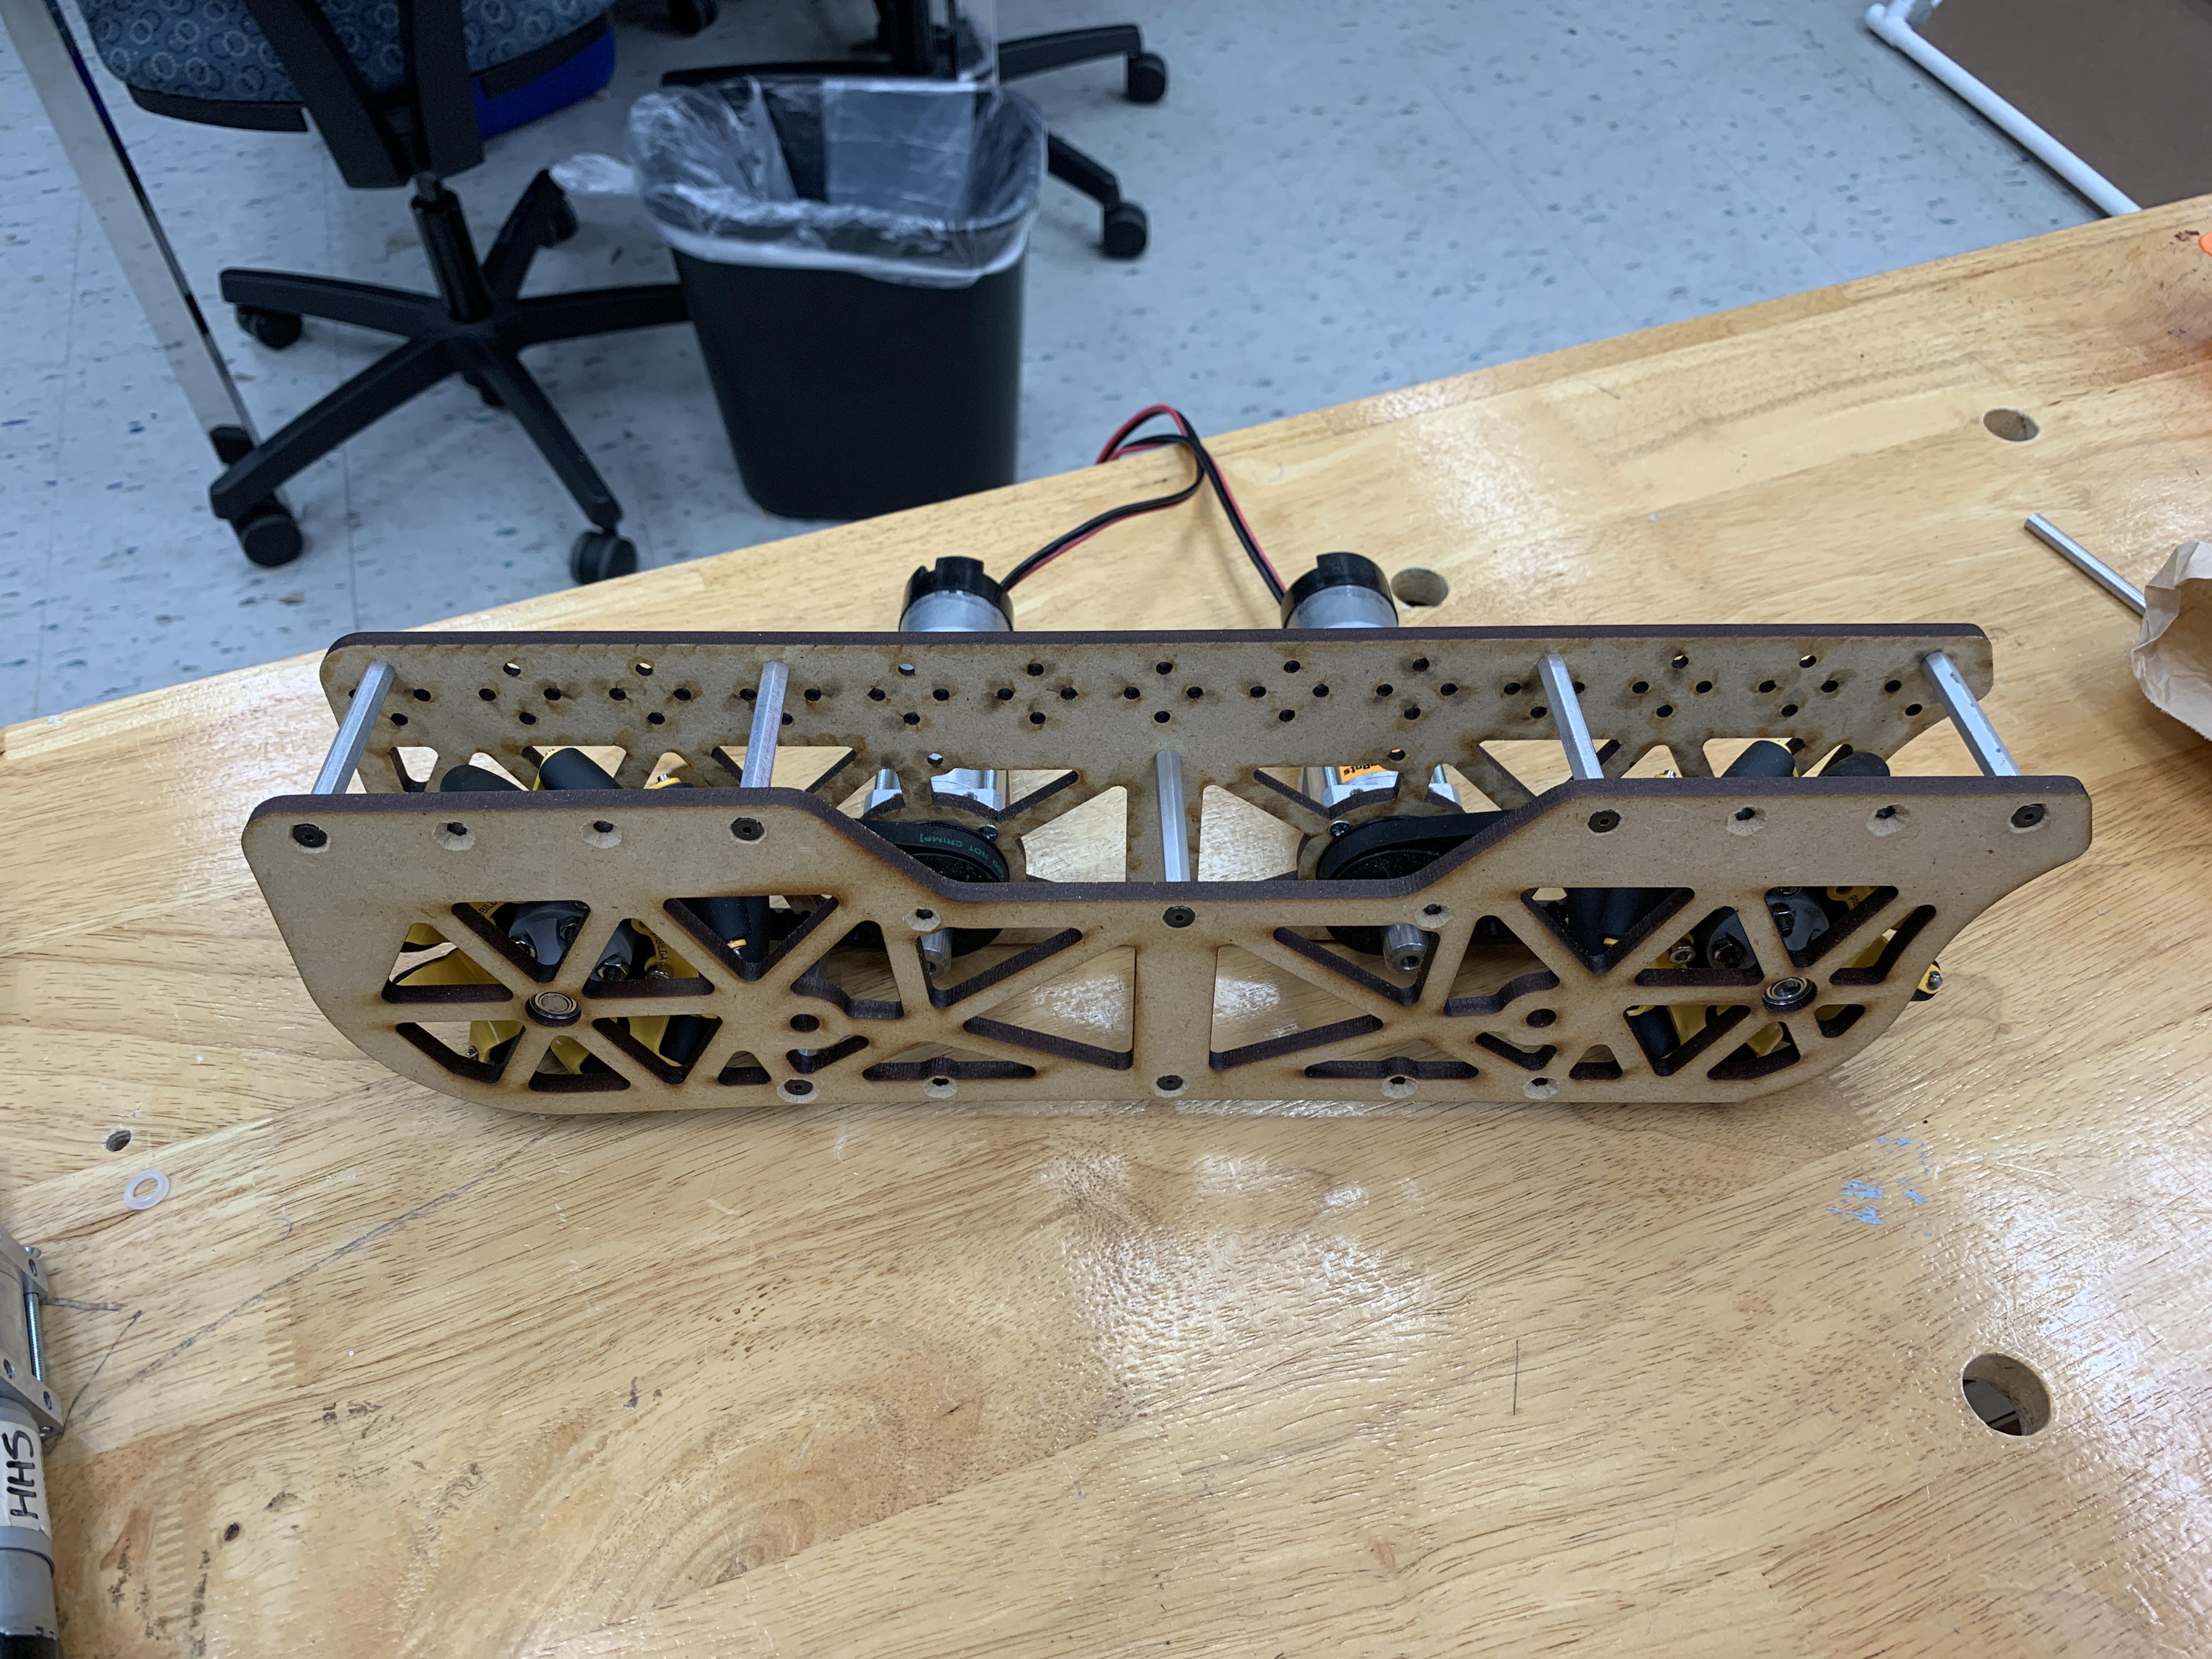
\includegraphics[width=0.9\textwidth, angle=0]{Meetings/July/07-21-21/drivetrain_7-20-21-NathanForrer.jpg}
\caption{First half of the drivetrain.}
\label{fig:pic1}
\end{figure}